\section{Обзор литературы}

\subsection{Различные типы хромофоров}

\subsection{Споряженные донорно-акцепторные (\emph{push-pull}) хромофоры}

Споряженные донорно-акцепторные хромофоры представляют большой интерес из-за их электрооптических свойств: система сопряженных двойных связей позволяет образовать низколежащую \ac{lumo} провести внутримолекулярный перенос заряда. Они применяются в таких областях, как органическая электроника, электрооптика, фотовольтаика~\cite{Bures2014a}.

\begin{figure}
    \centering
    
\includegraphics{sections/literature/img/D-p-A_chromophores.eps}
    \caption{Общая структура \emph{push-pull} хромофоров}
\end{figure}

\subsection{Хромофоры с донорным блоком на основе триарилпиразолинов}

\subsection{Различные акцепторные блоки}

\begin{figure}
    \centering
    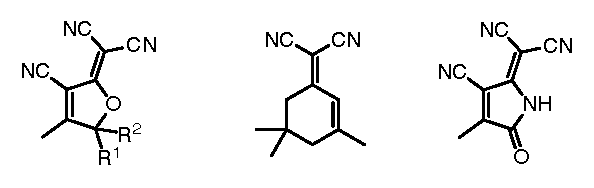
\includegraphics{sections/literature/img/acceptors.eps}
    \caption{Различные акцепторы~\cite{Dalton2010a}}
\end{figure}

\subsection{Влияние дендроидного заместителя}

\subsection{Нелинейные хромофоры и их применение}


\subsection{Подходы к синтезу триарилпиразолинов}

\begin{figure}
    \centering
    
\includegraphics{sections/literature/img/pyrazoline_structure.eps}
    \caption{Структура и нумерация атомов 2-пиразолина}
\end{figure}

Основным способом синтеза 1,\,3,\,5-триарилпиразолинов является реакция конденсации халконов с фенилгидразинами. Установлено, что обычно первым вступает в реакцию вторичный атом азота, реагируя с двойной связью халкона. Далее второй атом азота реагирует с карбонильной группой, замыкая пиразолиновый цикл. Этот подход является достаточно общим, как было показано в работе~\cite{Powers1998}, где таким способом была получена библиотека из \num{7680} соединений с различными заместителями во всех трех ароматических ядрах.

\begin{scheme}
    \centering
    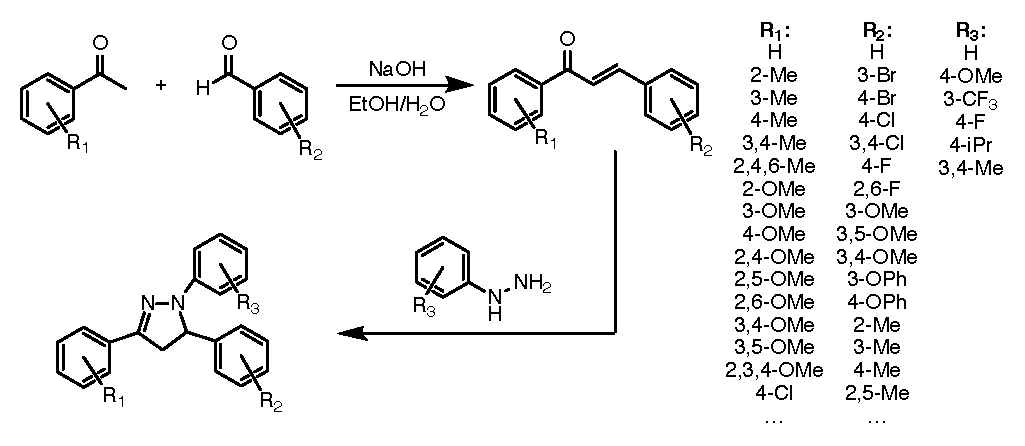
\includegraphics{sections/literature/img/pyrazolines_common.eps}
    \caption{Cинтез триарилпиразолинов с использованием халконов}
\end{scheme}

Второй способ синтеза пиразолинов использует [3 + 2] циклоприсоединение илидов азометиновых иминов к алкинам. Использование хиральных комплексов металлов в качестве катализаторов позволяет стереоселективно получать энантиомерно чистые пиразолины. Циклоприсоединение илидов азометиновых иминов к алкенам дает полностью насыщенные аналоги пиразолинов~--- пиразолидины~\cite{Groselj2018}.

\begin{scheme}
    \centering
    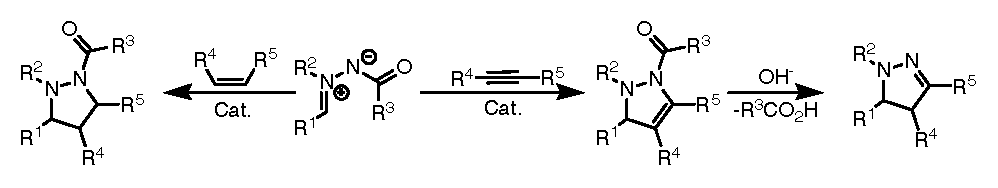
\includegraphics{sections/literature/img/pyrazolines_cycloaddition.eps}
    \caption{Синтез триарил пиразолинов с использовнием [3 + 2] циклоприсоединения}
\end{scheme}